\documentclass[paper=A4, ngerman, fontsize=12pt]{article}
\usepackage{geometry}
\geometry{
	a4paper,
	left=25mm,
	right=35mm,
	top=25mm,
	bottom=35mm,
}
\usepackage{setspace}
\onehalfspacing
\usepackage{babel}
\usepackage{fontspec}
\usepackage{microtype}
\usepackage{selnolig}
\usepackage{csquotes}
\usepackage{graphicx}
\usepackage{booktabs}

\begin{document}
	\thispagestyle{empty}
	{\large\noindent
		FAU Erlangen-Nürnberg
		
		\medskip\noindent
		Department Germanistik \& Komparatistik
		
		\medskip\noindent
		Lehrstuhl für Korpus- und Computerlinguistik
		
		\medskip\noindent
		Grundlagen der Computerlinguistik III
		
		\medskip\noindent
		Wintersemester 2022/2023
		
		\medskip\noindent
		Prof. Dr. Stephanie Evert
	}
	
	\vspace*{\fill}
	\begin{center}
		{\large Named Entity Recognition in juristischen Urteilen mit traditionellen maschinellen Lernverfahren}
		
		\medskip\noindent
		{\large
			\textit{Projektbericht für \enquote{Grundlagen der Computerlinguistik III}}
		}
		
	\end{center}
	\vspace*{\fill}
	
	
	\mbox{}
	\vfill
	{\large
		\noindent
		Xinyao Lu
		
		\medskip\noindent
		Matrikelnummer: 23008498
		
		\medskip\noindent
		xinyao.lu@fau.de
		
		\medskip\noindent
		Computerlinguistik/Germanistik
		
		\medskip\noindent
		3. Fachsemester
		
		\medskip\noindent
		Abgabe: 31.03.2023
	}
	
	\clearpage
	
	
	\thispagestyle{empty}
	\tableofcontents
	\listoffigures
	\listoftables
	
	\clearpage
	
	\section{Zusammenfassung}
	\noindent
	Als Seminarprojekt für die Lehrveranstaltung Grundlagen der Computerlinguistik III an der FAU Erlangen-Nürnberg wird das \enquote{Sub-task B: Legal Named Entities Extraction} vom \enquote{SemEval-2023, Task 6: LegalEval: Understanding Legal Texts} ausgewählt.\footnote{Link zum Task: https://sites.google.com/view/legaleval/home\#h.fbpoqsn0hjeh}
	
	Die Datensätze dieser Aufgabe sind englischsprachige juristische Urteile in Indien. Im Projekt werden nur traditionelle maschinelle Lernverfahren verwendet. Trotzdem hat das Projekt auch ein befriedigendes Ergebnis (75\% strenger f1-Score) mit mindestens 47\% Recall bei allen Hauptkategorien (Support >= 50) im Developing Datensatz bekommen. 
	
	\index Der gesamte Code dieses Projekts in verschiedenen Modulen mit der Pipeline und ihrer Visualisierung kann im GitHub-Repository \enquote{LegalNER\_GdCL\_III\_Projekt} gefunden werden.\footnote{Link zum Repository: https://github.com/cometbridge1998/LegalNER\_GdCL\_III\_Projekt}
	
	\section{LegalNER: Projektbeschreibung}
	\subsection{Aufgaben der allgemeinen Named Entity Recognition}
	\noindent
	Named Entity Recognition ist ein grundlegender Bereich des Natural Language Processings, der viele fortschrittliche semantische Analysen des Texts, beispielsweise Informationsextraktion, ermöglicht. Die sogenannten Named Entities sind \enquote{Objekte in der realen Welt, z. B. eine Person, ein Ort, eine Organisation, ein Produkt, etc., die mit einem Eigenname referenziert werden können.}\footnote{https://en.wikipedia.org/wiki/Named\_entity: \enquote{In information extraction, a named entity is a real-world object, such as a person, location, organization, product, etc., that can be denoted with a proper name.}}
	
	Die Aufgabe eines Named Entity Recognition Programms (kurz: NER) ist, solche Einheiten aus unterschiedlichen Textarten zu erkennen und in Kategorien zu ordnen. Da die Verteilung von den Named Entities in unterschiedlichen Textarten sehr unterschiedlich sein kann und unterschiedliche Klassifikationen in spezifischen Anwendungen angefordert werden, sind die allgemeinen NER Modelle nicht immer geeignet für alle Aufgaben. Dadurch entsteht die Notwendigkeit, spezifische Programme für bestimmte Aufgaben zu entwickeln. 
	
	\subsection{Spezielle Aufgaben der LegalNER}
	\noindent
	NER in den juristischen Unterlagen (LegalNER) ist eine dieser Aufgaben, die ein spezifisches Programm auffordern.  \enquote{Named Entities in juristischen Texten sind etwas anders und feiner als normale verwendete Named Entities ...}\footnote{[Named Entity Recognition in Indian court judgments](https://aclanthology.org/2022.nllp-1.15) (Kalamkar et al., NLLP 2022): \enquote{Named Entities in legal texts are slightly different and more fine-grained than commonly used named entities like Person, Organization, Location etc.}} Viele Kategorien in der LegalNER wie \enquote{JUDGE} (Richter), \enquote{PETITIONER} (Kläger), \enquote{RESPONDENT} (Angeklagter) werden in meisten allgemeinen NER Programmen nicht voneinander unterschieden oder werden vernachlässigt wie \enquote{STATUTE} (Bestimmung), \enquote{PRECEDENT} (Präzedenzfall). Außerdem werden komplexerer Satzbau und eine große Menge von Fachbegriffen in den juristischen Unterlagen häufig verwendet. 
	
	\indent
	Juristische Urteile bestehen normalerweise aus zwei Teilen, \enquote{preamble} (Präambel) und \enquote{judgement} (Urteil). \enquote{Die Präambel eines Urteils enthält formatierte Metadaten wie Namen der Parteien, des Richters, der Rechtsanwälte, das Datum, das Gericht usw. Der folgende Text wird \enquote{Urteil} genannt.}\footnote{[Named Entity Recognition in Indian court judgments](https://aclanthology.org/2022.nllp-1.15) (Kalamkar et al., NLLP 2022): \enquote{The preamble of a judgment contains formatted metadata like names of parties, judges, lawyers, date, court etc. The text following the preamble till the end of the judgment is called "judgment".}} Im Datensatz vom Shared-Task werden Präambeln und Urteile getrennt gespeichert. Die Verteilung der Named Entities in der Präambel ist meistens viel dichter als im darauf folgenden Urteil. Deswegen sind die Datensätze für Urteile durch Auswahl der \enquote{dicht besetzten} Sätze \enquote{intensiviert}. In diesem Projekt werden nur die Datensätzen für Urteile verwendet. 
	
	\subsection{Erkennen und Einordnen: doppelte Aufgaben der NER}
	\noindent
	Die Schwierigkeit einer NER-Aufgabe liegt darin, dass sie nicht nur die richtige Klassifikation, sondern auch die genaue Erkennung der Entities (nicht länger, nicht kürzer) benötigt. Allerdings ist es für ein traditionelles Lernverfahren notwendig, Texte in Token zu splitten (Tokenisierung) und demnächst in eine Matrix, die als Eingabe für das maschinelle Lernen dient, umzuwandeln. Eine Entity entspricht normalerweise mehrere Tokens. Für einige besonders lange Arten von Entities wie \enquote{PRECEDENT} und \enquote{STATUTE}, sind Entities mit mehr als 10 Tokens  nicht selten. 
	
	\indent
	Wegen der unterschiedlichen Längen der Entities entsteht die \enquote{BIO} Tagging-Norm für NER-Aufgaben. Denjenigen Tokens, die sich am Anfang von einer Entity befinden, wird ein \enquote{B-} (\enquote{Beginning}) Label gegeben. \enquote{I-} Labels (\enquote{Insider}) markieren alle Tokens nach dem ersten Token in einer Entity. \enquote{O} (\enquote{Outsider}) Labels entsprechen allen Tokens, die sich in keiner Entity befinden. ( s. Tabelle 1: \enquote{BIO} Tagging-Norm ) Im Datensatz gibt es keine Überschneidung von den Labels. Jedes Token oder Zeichen befindet sich in maximal einer Entity.
	
	\begin{table}
		\begin{center}
			\begin{tabular}{@{}| c | c | @{}}
				\toprule
				Token & Label   \\ \midrule
				\hline
				... & ...  \\ \midrule
				of & o  \\ \midrule
				Hongkong & B-ORG \\   \midrule
				Bank & I-ORG \\   \midrule
				... & ... \\  \bottomrule
			\end{tabular}
			\caption{ \enquote{BIO}-Tagging-Norm}
		\end{center}
	\end{table}	
	
	\section{Vorbereitung zum maschinellen Lernen}
	
	\subsection{Tokenisierung}
	\noindent
	Die vom Shared Task angebotenen Datensätze sind in JSON Objekten gespeichert. Die annotierten Labels sind mit \enquote{String Slices} angegeben. Z. B.: 
	
	\indent
	 \enquote{... Hongkong Bank ...}
	 
	 \indent
	\{ \enquote{value}: \{ \enquote{start}: 90, \enquote{end}: 103 \}, \enquote{text}: \enquote{Hongkong Bank}, \enquote{labels}: [\enquote{ORG}] \} 
	
	Der erste Schritt dieses Projekts ist, alle Texte mit ihren Annotationen in ein Dataframe, das fortschrittliche Verarbeitungen vereinfacht, umzuwandeln. Jede Zeile im Dataframe entspricht einem Token in den Texten. Jede Spalte speichert eine Eigenschaft der Tokens wie \enquote{SentenceNr} (Satznummer), \enquote{Label} (nach der \enquote{BIO}-Tagging-Norm) etc. 
	
	\indent
	Ein kleines Problem bei der Umwandlung des Textes in das Dataframe ist, dass die Norm der Tokenisierung nicht vernachlässigt werden darf, besonders wenn die Satzzeichen eine Rolle zur semantischen Interpretation des Satzes spielen. Wenn z. B. ein Punkt am Ende eines Aussagesatzes steht, soll er als getrenntes Token behandelt werden. Im Gegensatz dazu, handelt es sich bei dem Punkt um Kennzeichen für eine Abkürzung, soll er mit den vorangehenden Buchstaben ein ganzes Token bilden. 
	
	\indent
	Das Projekt hat für die Tokenisierung den \enquote{TreebankWordTokenizer} vom Paket \enquote{nltk} gewählt.\footnote{Link zum Dokument vom Tokenizer: Zitat aus: https://www.nltk.org/api/nltk.tokenize.TreebankWordTokenizer.html} Die Qualität der Tokenisierung wird durch den Vergleich zwischen dem Goldstandard nach Annotation und den \enquote{detokenisierten} Texten, die Wiederzusammenstellung der Texte in den Entities nach der Tokenisierung, überprüft. Es wird also verglichen, ob die Texte der Entities (inkl. Satzzeichen) bei der Tokenisierung geändert werden. Nach der Überprüfung gibt es insgesamt nur 7 Entities im gesamten Trainings- und Developingsdatensatz, die wegen der Tokenisierung leicht geändert werden. Vier Änderungen behandeln die Löschung eines Bindestrichs. Durch diese geringe Menge von Fehlern sollte kein spürbarer Effekt bei der endgültigen Evaluation entstehen. Spezifische Reports über alle Tokenisierungsfehler können in \enquote{tokenizing\_report\_train(dev).txt} aus dem Projektsrepository gefunden werden.

	\subsection{Part-of-Speech-Tagging}
	\noindent
	\enquote{Unter Part-of-speech-Tagging (POS-Tagging) versteht man die Zuordnung von Wörtern und Satzzeichen eines Textes zu Wortarten (englisch part of speech).}\footnote{https://de.wikipedia.org/wiki/Part-of-speech-Tagging} Weil die Entities häufig bestimmten Satzteilen entsprechen, werden POS-Tags in das Dataframe hinzugefügt. 
	
	\indent
	Zwei POS-Tagger werden vom Projekt benutzt. Der erste Tagger ist der Standardtagger von nltk (ein vortrainierter PerceptronTagger). Dieser Tagger gibt einen POS-Tag zu jedem Token zurück. Dadurch werden null-Werte bei seltenen Tokens im Dataframe vermieden. Der zweite Tagger ist ein mit \enquote{Penn treebank} konfigurierter TreeTagger. Ein Vorteil vom TreeTagger liegt darin, dass er neben POS-Tags zusätzlich die \enquote{Lemmata} (Stammformen) von Tokens liefert. Der Zusatz der Lemmata in das Dataframe soll nach Vorstellung des Entwicklers die Störung von verschiedenen Flexionsformen beseitigen und dadurch die Stabilität des Modells fördern. Im Gegensatz zum Standardtagger von nltk liefert TreeTagger keinen Tag und kein Lemma für unbekannte Tokens. Bei solchen Tokens, die weder Tag noch Lemma vom TreeTagger bekommen, sind die leeren Zellen mit \enquote{0} gefüllt. Spezifische Einzelheiten über Installierung und Konfiguration des TreeTaggers sind im File \enquote{README.md} vom Projektrepository angegeben. 
	
	\subsection{Feature Matrix}
	\noindent
	Feature Matrix soll dem maschinellen Lernmodell zusätzliche Informationen neben den schon vorhandenen Tokens, POS-Tags und Lemmata liefern, besonders die \enquote{Kontextinformationen}. Mit \enquote{Kontext} sind die umgebenden Tokens und ihre Eigenschaften gemeint. Die Auswahl der \enquote{Features} muss normalerweise empirisch bestimmt werden, d. h., die beste Feature Matrix muss durch Ausprobieren unterschiedlicher Kombinationen festgestellt werden. 
	
	\indent
	Um das Textdataframe in eine für maschinelles Lernverfahren geeignete Matrix umzuwandeln, werden drei \enquote{CountVectorizer} verwendet, die jeweils mit Tokens, POS-Tags und Lemmata im Trainingsdatensatz initialisiert werden. 
	
	\indent
	Das Dataframe wird nach \enquote{SentenceNR} (Nummer des Satzes) gruppiert. Als Kontextinformationen eines Tokens werden nur Tokens im selben Satz berücksichtigt. Als Kontextinformationen von den an der Satzgrenze liegenden Tokens werden \enquote{Paddings}, statt Tokens in den vorangehenden oder folgenden Sätzen, gegeben. Z. B.:
	
	\indent
	Für das vorletzte Token \enquote{copy} im Satz: \enquote{ ... on that photo copy . },
	
	\indent
	L1 Token is \enquote{photo}. L2: \enquote{that}, R1: \enquote{.} und R2: \enquote{·} (Paddingszeichen).
	
	\indent
	Nach systematischen Vergleichen hat die Feature Matrix mit den folgenden Spalten bei einem \enquote{LinearSVC}-Modell aus dem Paket scikit-learn bestes Ergebnis erreicht:
	
	\indent
	Token, POS-Tag und Lemma vom Token selbst und von deren L1, L2, R1, R2 Nachbartokens. 
	
	\indent
	Affixe und weitere Eigenschaften von den Tokens können das Ergebnis nicht verbessern. Sie führen nur zu einer höheren Überanpassung an den Trainingsdatensatz. Der Versuch mit einer dynamischen Feature Matrix dem Modell mit den (vorhergesagten) Labels vorangehender Tokens zu bieten, hat das Ergebnis sondern wesentlich verschlechtert. 
	
	\subsection{Model Selection}
	\noindent
	Um das möglichst beste Ergebnis zu erreichen, werden zwei Modelle traditioneller Lernverfahren mit \enquote{Parameter Finetuning} (Ausprobieren unterschiedlicher Parameterkombinationen) verwendet. 
	
	\indent
	Das LinearSVC-Modell aus scikit-learn hat mit folgenden Parametern einen strengen f1-score von 67\% bekommen. (Evaluationskriterien werden in \enquote{4.1 Zwei Methoden zur Evaluation} erklärt.)
	
	\indent
	\{\enquote{C}: 0.35, \enquote{class\_weight}: None, \enquote{loss}: \enquote{hinge}, \enquote{penalty}: \enquote{l2}\}
	
	\indent
	Das \enquote{sklearn\_crfsuite}-Modell ist eine Erweiterung des scikit-learn-Pakets. Mit der Stärke, die Abfolge der Labels zu lernen, ist das Modell besonders für NER-Aufgaben geeignet. Das Modell bietet vergleichbare Funktionen wie scikit-learn, welche die Anpassung zu anderen Programmteilen erleichtern. Mit der \enquote{word2features}-Funktion des sklearn\_crfsuite-Modells wird eine Standard-Feature-Matrix erzeugt. Mit dieser Standard-Matrix und den Hyperparametern
	
	\indent
	 \{\enquote{c1}: 0.173, \enquote{c2}: 0.203\}
	 
	 \indent
	 hat das Modell ein wesentlich besseres Ergebnis als das LinearSVC-Modell erreicht: strenger f1-score: 75\%.
	 
	\section{Evaluation und Fehleranalyse}
	
	\subsection{Zwei Methoden zur Evaluation}
	\noindent
	Da jede Zeile in der Eingabematrix einem einzelnen Token (statt einer Entity) entspricht, sind die vorhergesagten Labels (y\_predict) auch eine Liste von Labels für einzelne Tokens. Die einfache Evaluation auf der Token-Ebene (Wie viele Tokens bekommen die richtigen Labels?) darf nicht als das endgültige Ergebnis eines NER-Modells zählen. Wie in \enquote{2.3 Erkennen und Einordnen: doppelte Aufgaben der NER} hingewiesen wird, muss eine ernsthafte Evaluation auf der Entity-Ebene auch die beiden Aufgaben eines NER-Modells bewerten. Nach diesem speziellen Anspruch werden auch zwei Methoden zur Evaluation im Projekt definiert. 
	
	\indent
	Der Klassifizierungsreport zeigt die Genauigkeit bei der Klassifikation der Entities, d. h., wie viele derjenigen Tokens, die mit richtigen Längen (span) erkannt werden, werden mit richtigen Labels eingeordnet. Diese Methode reflektiert nur die Genauigkeit der Einordnung der Entities, beispielsweise, ob \enquote{Hongkong Bank} eine \enquote{ORG} (organization) oder eine \enquote{GPE} (geopolitical entity) ist.
	
	\indent
	Der Recognition-Report zeigt die Genauigkeit eines NER-Modells sowohl bei der Erkennung als auch bei der Einordnung der Entities. Um als eine richtige Vorhersage in diesem Report zu zählen, muss die Entity mit vollständiger Länge erkannt und auch in die richtige Kategorie eingeordnet werden. Der f1-score vom Recognition-Report wird vom Organisator des Shared-Tasks als \enquote{strict f1-score} (strenger f1-score) bezeichnet.  
	
	\indent
	Wenn man die zwei Reports eines gleichen Modells vergleicht, hat der Klassifizierungsreport immer einen höheren f1-score (\enquote{harmonic mean} von precision und recall), aber niedrigeren support (Support zeigt die Anzahl der beteiligten Entities in der Evaluation). Das Phänomen ist leicht erklärbar. Der Klassifizierungsreport bewertet nur die Genauigkeit der einzelnen Aufgabe \enquote{Einordnung}, während der Recognition-Report beide Aufgaben bewertet. Je höher der support im Klassifizierungsreport eines Modells ist, desto mehr Entities werden vollständig erkannt. 
	
	\indent
	Die beiden Modelle erreichen über 93\% beim gewichteten F1-score in den Klassifizierungsreports. Allerdings sind die F1-scores in den Recognition-Reports mit Abstand niedriger. Dadurch kann man feststellen, dass die meisten Fehler aus der unvollständigen Erkennung der Längen von Entities entstehen, d. h., solange eine Entity vollständig gefunden wird, ist die Einordnung viel leichter. 
	
	\begin{figure}
		\begin{center}
			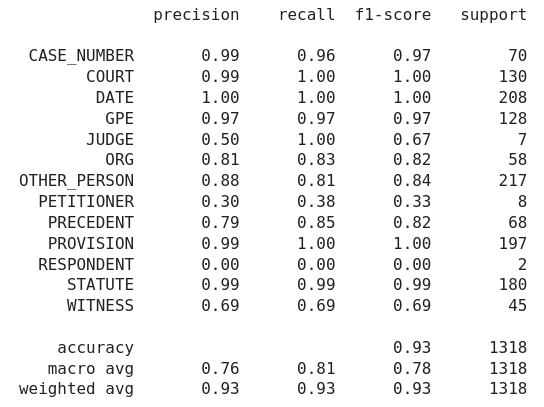
\includegraphics[width=8cm]{Illustrations/svc_classify.png}
			\caption{Klassifizierungsreport vom LinearSVC Modell}
			\label{Klassifizierungsreport vom LinearSVC Modell}
		\end{center}
	\end{figure}

	\begin{figure}
		\begin{center}
			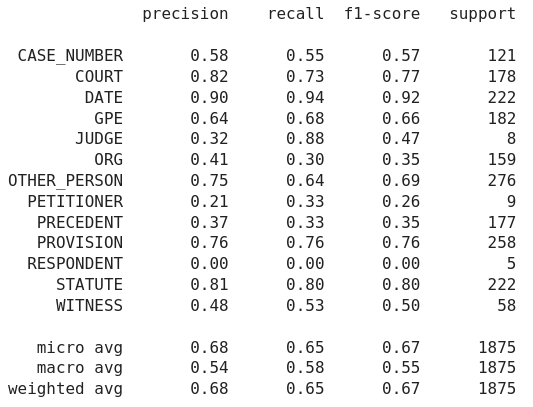
\includegraphics[width=8cm]{Illustrations/svc_recognition.png}
			\caption{Recognitionsreport vom LinearSVC Modell}
			\label{Recognitionsreport vom LinearSVC Modell}
		\end{center}
	\end{figure}

	\subsection{Zwei Methoden zur Evaluation}
\begin{figure}
	\begin{center}
		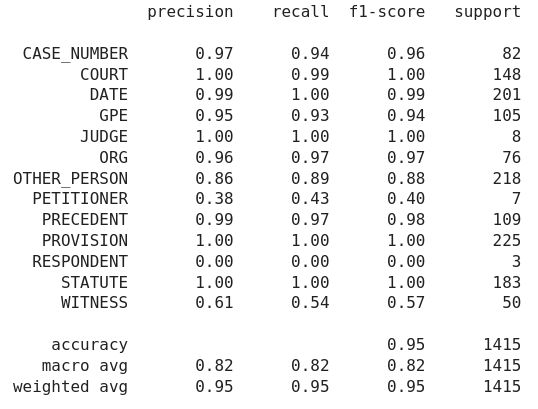
\includegraphics[width=8cm]{Illustrations/crf_classify.png}
		\caption{Klassifizierungsreport vom crfsuite Modell}
		\label{Klassifizierungsreport vom crfsuite Modell}
	\end{center}
\end{figure}

\begin{figure}
	\begin{center}
		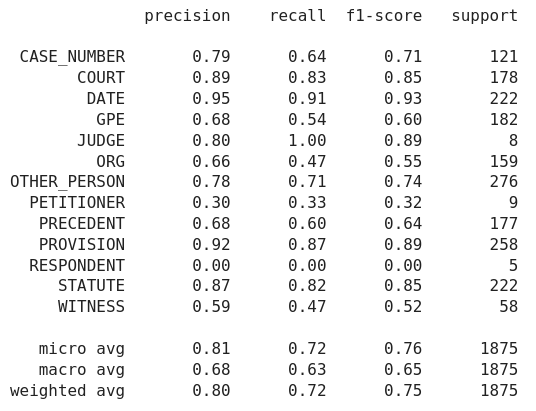
\includegraphics[width=8cm]{Illustrations/crf_recognition.png}
		\caption{Recognitionsreport vom crfsuite Modell}
		\label{Recognitionsreport vom crfsuite Modell}
	\end{center}
\end{figure}

	\subsection{Confusion Matrix}
	\noindent
	Die Confusion-Matrix ist eine im scikit-learn eingebaute Funktion, um die falschen Entscheidungen eines Modells herauszufinden. Da sich eine Confusion-Matrix von allen 13 Kategorien (13*13) schwer in einer Abbildung zeigen lässt,  werden die Labels in drei Hauptklassen klassifiziert:
	
	\clearpage
	\indent
	\enquote{natural\_person}: [ \enquote{JUDGE}, \enquote{OTHER\_PERSON}, \enquote{PETITIONER}, \enquote{RESPONDENT}, \enquote{WITNESS} ]
	
	\indent
	\enquote{formats} = [ \enquote{CASE\_NUMBER}, \enquote{PRECEDENT}, \enquote{PROVISION}, \enquote{STATUTE}, \enquote{DATE} ]
	
	\indent
	\enquote{juridical\_person} = [ \enquote{COURT}, \enquote{GPE}, \enquote{ORG} ]
	
	\indent
	Die Confusion-Matrix jeder oben genannten Klasse kann einzeln dargestellt werden. Abbildung 5 zeigt die Confusion-Matrix von der Klasse \enquote{natural\_person} mit dem crfsuite-Modell. 
	
	\begin{figure}
		\begin{center}
			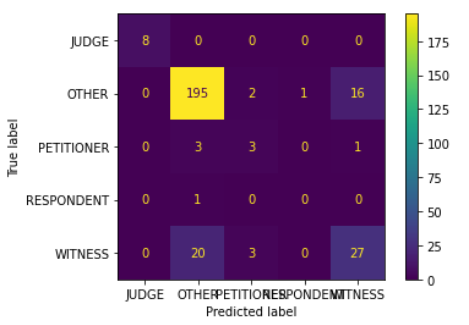
\includegraphics[width=8cm]{Illustrations/confusion_matrix.png}
			\caption{Confusion Matrix von der Klasse natural person}
			\label{Confusion Matrix von der Klasse natural person}
		\end{center}
	\end{figure}

	\subsection{Fehleranalyse mit dem Beispiel der Präzedenzfälle}
	\noindent
	Eine Fehleranalyse, d. h. eine inhaltliche Überprüfung des Lernergebnisses, ist notwendig, um weitere Möglichkeit zur Verbesserung des Modells herauszufinden.  
	
	\indent
	Durch einen Vergleich der Ergebnisse jeder Kategorien von den zwei Modellen kann man feststellen, dass das LinearSVC-Modell eine ähnliche Leistung bei den meisten Kategorien mit durchschnittlich kürzeren Längen (\enquote{COURT}, \enquote{DATE}, \enquote{GPE}, \enquote{STATUTE}) wie das crfsuite-Modell erreicht.\footnote{Ausschließlich den Kategorien in der Klasse \enquote{natural\_person}. Sie werden in \enquote{4.4.2 Beispiel II: natural\_person: eine unausgewogene Klasse} zusätzlich diskutiert.} Allerdings bei längeren Kategorien, wie \enquote{ORG}, \enquote{PRECEDENT}, \enquote{PROVISION}, hat das crfsuite-Modell ein eindeutig besseres Ergebnis bekommen. 
	
	\indent
	Bei der Kategorie \enquote{PRECEDENT} gibt es den größten Unterschied der Ergebnisse aus den beiden Modellen.\footnote{LinearSVC-Modell: f1-Score 85\% bei der Klassifizierung, strenger f1-Score 33\% ber der Recognition; crfsuite-Modell: entsprechend 98\% und 64\%.} Die häufigsten Einordnungs- oder Erkennungsfehler bei der \enquote{PRECEDENT} Klasse können mindestens in vier Typen zusammengefasst. 
	
	\medskip
	\indent
	Typ 1: Personennamen in den \enquote{PRECEDENT}
	
	\indent
	Da die Präzedenzfälle in den juristischen Unterlagen häufig nach den beteiligten Personen des Verfahrens genannt werden, ist es eine Herausforderung für die Modelle, zwischen den Namen innerhalb eines \enquote{PRECEDENT} und Namen der natürlichen Personen als einzelne Entities zu unterscheiden. (Als Beispiel s. Tabelle 2: \enquote{OTHER\_PERSON} vs. \enquote{PRECEDENT})
	
\begin{table}
	\begin{center}
		\begin{tabular}{@{}| c | c c | @{}}
			\toprule
			Token & True& Pred   \\ \midrule
			\hline
			... & ... & ... \\ \midrule
			Court & o & o \\   \midrule
			in & o & o \\   \midrule
			Vikram & B-PRECEDENT & B-OTHER\_PERSON  \\  \midrule
			Singh &  I-PRECEDENT & I-OTHER\_PERSON  \\   \midrule
			@ &  I-PRECEDENT& I-PRECEDENT \\   \midrule
			Vicky & I-PRECEDENT & I-PRECEDENT \\  \midrule
			v. &  I-PRECEDENT & I-PRECEDENT \\   \midrule
			Union & I-PRECEDENT  & I-PRECEDENT \\   \midrule
			of & I-PRECEDENT  & I-PRECEDENT \\  \midrule
			India16 & I-PRECEDENT  &  I-PRECEDENT  \\   \midrule
			wherein & o & o \\   \midrule
			it & o & o \\ \midrule
			... & ... & ... \\ \bottomrule
		\end{tabular}
		\caption{ \enquote{OTHER\_PERSON} vs. \enquote{PRECEDENT} }
	\end{center}
\end{table}


	\medskip
	\indent
	Typ 2: Namen der juristischen Personen in den \enquote{PRECEDENT}
	
	\indent
	Das Modell hat häufig auch Namen der juristischen Personen in den Entities als einzelne Entities ausgefiltert. (Als Beispiel s. Tabelle 3: \enquote{GPE} vs. \enquote{PRECEDENT}) 
	
		\begin{table}
	\begin{center}
		\begin{tabular}{@{}| c | c c | @{}}
			\toprule
			Token & True& Pred   \\ \midrule
			\hline
			... & ... & ... \\ \midrule
			case & o & o \\ \midrule
			of & o & o \\ \midrule
			Printpak & B-PRECEDENT & B-PRECEDENT \\   \midrule
			Machinery & I-PRECEDENT & I-PRECEDENT \\   \midrule
			v. & I-PRECEDENT & I-PRECEDENT  \\  \midrule
			Jay &  I-PRECEDENT & I-PRECEDENT \\ \midrule
			Kay &  I-PRECEDENT& I-PRECEDENT \\   \midrule
			Paper & I-PRECEDENT & I-PRECEDENT \\  \midrule
			Congeners & I-PRECEDENT & I-PRECEDENT \\  \midrule
			reported & I-PRECEDENT & I-PRECEDENT \\  \midrule
			in & I-PRECEDENT & I-PRECEDENT \\  \midrule
			AIR & I-PRECEDENT & I-PRECEDENT \\  \midrule
			, & I-PRECEDENT & I-PRECEDENT \\  \midrule
			1979 & I-PRECEDENT & I-PRECEDENT \\  \midrule
			Delhi & I-PRECEDENT & B-GPE \\  \midrule
			271 & I-PRECEDENT & I-PRECEDENT \\  \midrule
			has & o & o \\  \midrule
			also & o & o  \\  \midrule
			... & ... & ... \\  \bottomrule
		\end{tabular}
		\caption{ \enquote{GPE} vs. \enquote{PRECEDENT} }
	\end{center}
\end{table}	
	
	\medskip
	\indent
	Typ 3: \enquote{Keine Erkennung des \enquote{B-Labels}}
	
	\indent
	Nach der \enquote{BIO}-Tagging-Norm muss das erste Token von der Entity mit dem \enquote{B-Label} gekennzeichnet werden, um die vorhergesagten Labels in eine Entity zu vereinigen. Weil jedes Token in den traditionellen Lernverfahren einzeln gelernt und vorhergesagt wird, gibt es keine Gewährleistung, dass jede vorhergesagte Entity mit einem \enquote{B-Label} beginnt. Manche Entities werden zwar in den (fast) genauen Längen erkannt und in die richtigen Kategorien eingeordnet, können sie allerdings noch nicht als eine richtige Recognition im strengen f1-Score zählen, wenn das erste Token nicht mit dem \enquote{B-Label} markiert wird oder ein beliebiges Token nach dem ersten Token ein \enquote{B-Label} bekommt. (Als Beispiel s. Tabelle 4: ohne \enquote{B-Label})
	
\begin{table}
	\begin{center}
		\begin{tabular}{@{}| c | c c | @{}}
			\toprule
			Token & True& Pred   \\ \midrule
			\hline
			... & ... & ... \\ \midrule
			option & o & o \\ \midrule
			but & o & o \\ \midrule
			( & B-PRECEDENT & o \\   \midrule
			2014 & I-PRECEDENT & I-PRECEDENT \\   \midrule
			) & I-PRECEDENT & I-PRECEDENT  \\  \midrule
			2 &  I-PRECEDENT & I-PRECEDENT \\ \midrule
			SCC &  I-PRECEDENT& I-PRECEDENT \\   \midrule
			1 & I-PRECEDENT & I-PRECEDENT \\  \midrule
			to &  o & o \\   \midrule
			... & ... & ... \\  \bottomrule
		\end{tabular}
		\caption{ohne \enquote{B-Label}}
	\end{center}
\end{table}	

	\medskip
	\indent
	Typ 4: Komma zwischen zwei \enquote{PRECEDENT}
	
	\indent
	Manchmal werden mehrere Präzedenzfälle mit einem Komma nebeneinander in den Urteilen zitiert. Solche Trennkommata lassen sich nicht einfach für die Modelle mit den Kommata innerhalb eines Präzedenzfalls unterscheiden. Die nebeneinander stehenden Präzedenzfällen werden deswegen nur als eine Entity erkannt. (Als Beispiel s. Tabelle 5: Komma zwischen zwei \enquote{PRECEDENT})

	\begin{table}
		\begin{center}
			\begin{tabular}{@{}| c | c c | @{}}
				\toprule
				Token & True& Pred   \\ \midrule
				\hline
				... & ... & ... \\ \midrule
				Ref. & o & o \\ \midrule
				Murarilal & B-PRECEDENT & I-PRECEDENT \\   \midrule
				v. & I-PRECEDENT & I-PRECEDENT \\   \midrule
				State & I-PRECEDENT & I-PRECEDENT  \\  \midrule
				of &  I-PRECEDENT & I-PRECEDENT \\ \midrule
				M.P. &  I-PRECEDENT& I-PRECEDENT \\   \midrule
				; & I-PRECEDENT & I-PRECEDENT \\  \midrule
				1980 & I-PRECEDENT & I-PRECEDENT \\  \midrule
				AIR & I-PRECEDENT & I-PRECEDENT \\  \midrule
				(  & I-PRECEDENT & I-PRECEDENT \\  \midrule
				SC & I-PRECEDENT & I-PRECEDENT \\  \midrule
				)  & I-PRECEDENT & I-PRECEDENT \\  \midrule
				531 & I-PRECEDENT & I-PRECEDENT \\  \midrule
				, & o & I-PRECEDENT \\  \midrule
				Alamgir & B-PRECEDENT & I-PRECEDENT \\  \midrule
				v. & I-PRECEDENT & I-PRECEDENT \\  \midrule
				State & I-PRECEDENT & I-PRECEDENT \\  \midrule
				(  & I-PRECEDENT & I-PRECEDENT \\  \midrule
				... & ... & ... \\  \bottomrule
			\end{tabular}
			\caption{ Komma zwischen zwei \enquote{PRECEDENT} }
		\end{center}
	\end{table}	

	\begin{figure}
		\begin{center}
			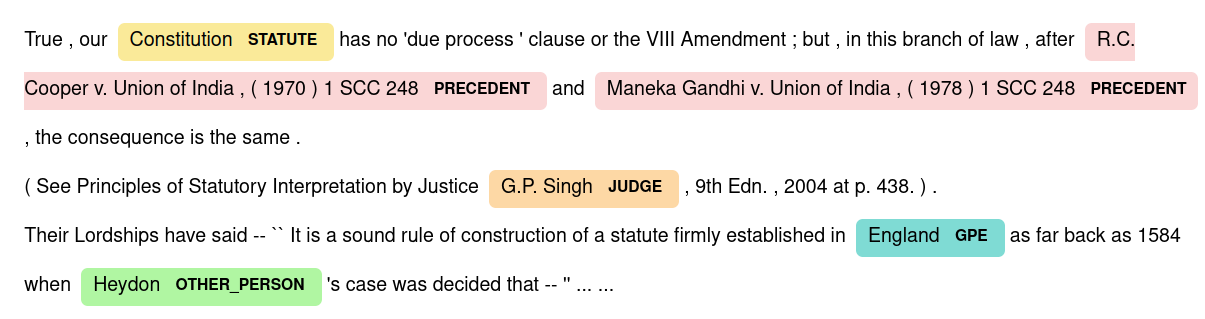
\includegraphics[width=15cm]{Illustrations/visualization.png}
			\caption{Visualisierungsbeispiel}
			\label{Visualisierungsbeispiel}
		\end{center}
	\end{figure}
	
	\clearpage
	
		
	\section*{Versicherung der selbstständigen Anfertigung}
	Der Unterzeichnete versichert, dass er die vorliegende schriftliche Hausarbeit selbstständig verfasst und keine anderen als die von ihm angegebenen Hilfsmittel benutzt hat. Die Stellen der Arbeit, die anderen Werken dem Wortlaut oder dem Sinne nach entnommen sind, wurden in jedem Fall unter Angabe der Quellen (einschließlich des World Wide Web und anderer elektronischer Text- und Datensammlungen) kenntlich gemacht. Dies gilt auch für beigegebene Zeichnungen, bildliche Darstellungen, Skizzen und dergleichen. 
	
	\begin{flushright}
		\medskip\noindent
		Erlangen, \today
		
		\noindent
		Unterschrift des Verfassers der Seminararbeit: 
		
		\noindent
		Xinyao Lu
	\end{flushright}
\end{document}